\section{Task 12}

During my verification process, I recalibrated the mean and covariance of each sensor to minimize the artificially introduced errors as much as possible. 


For each combination, I introduced three types of motion: primarily focused on rotation around the x-axis, primarily focused on rotation around the y-axis, and primarily focused on rotation around the z-axis.

They will be labeled as 1, 2, and 3 in the plots for each combination.


Before each experiment, sufficient time was given to the phone to initialize and calibrate the biases. This information can be observed from the graphs.

\subsection{All sensors}

\begin{figure}[H]
 \centering
 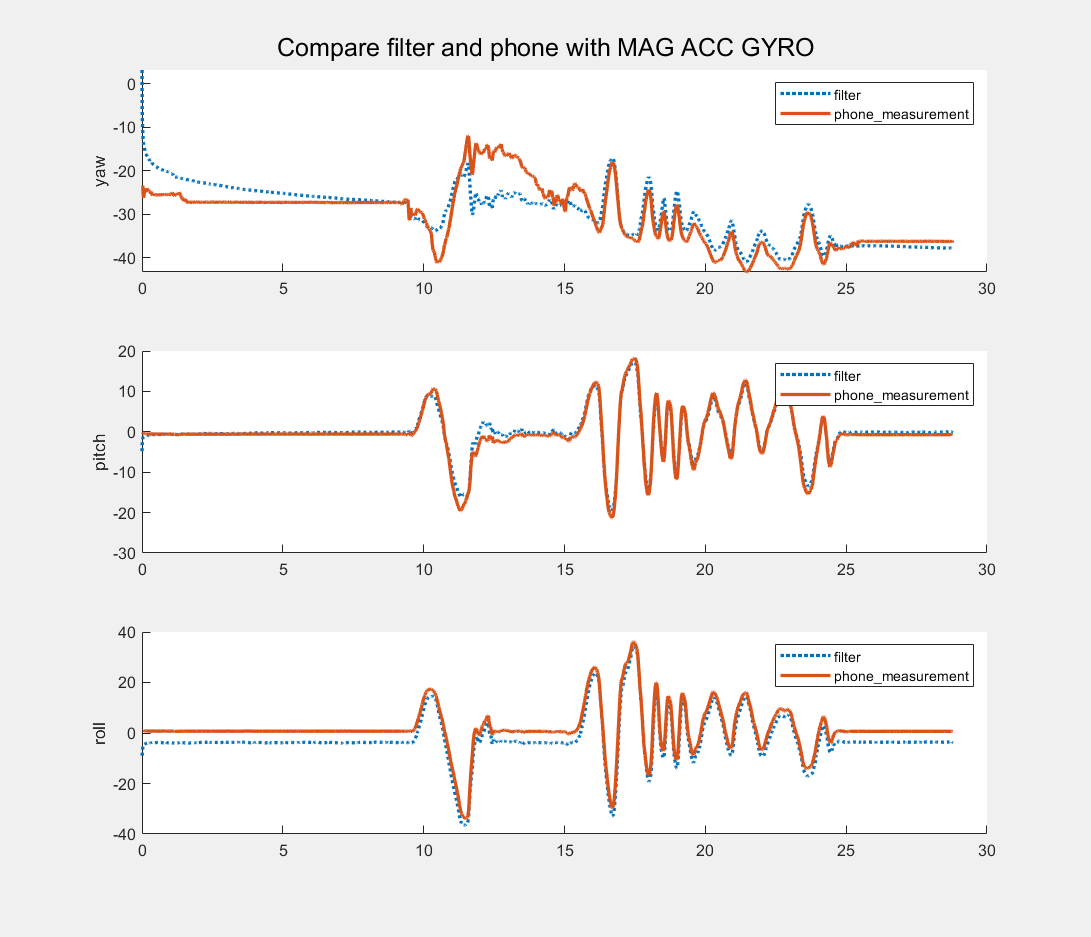
\includegraphics[width=0.7\textwidth]{images/allsensors1.png}
 \caption{All Sensors: 1}
 \label{all1}
\end{figure}

\begin{figure}[H]
 \centering
 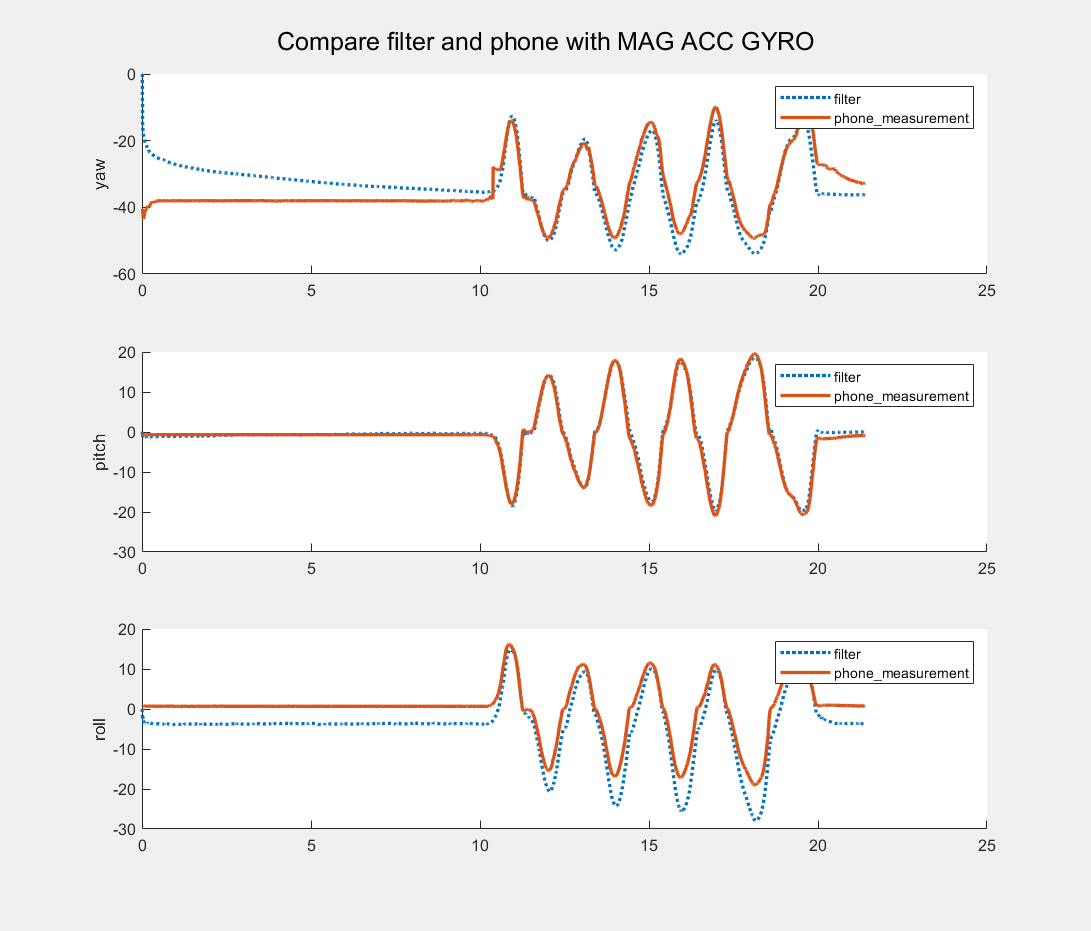
\includegraphics[width=0.7\textwidth]{images/allsensors2.png}
 \caption{All sensors: 2}
 \label{all2}
\end{figure}

\begin{figure}[H]
 \centering
 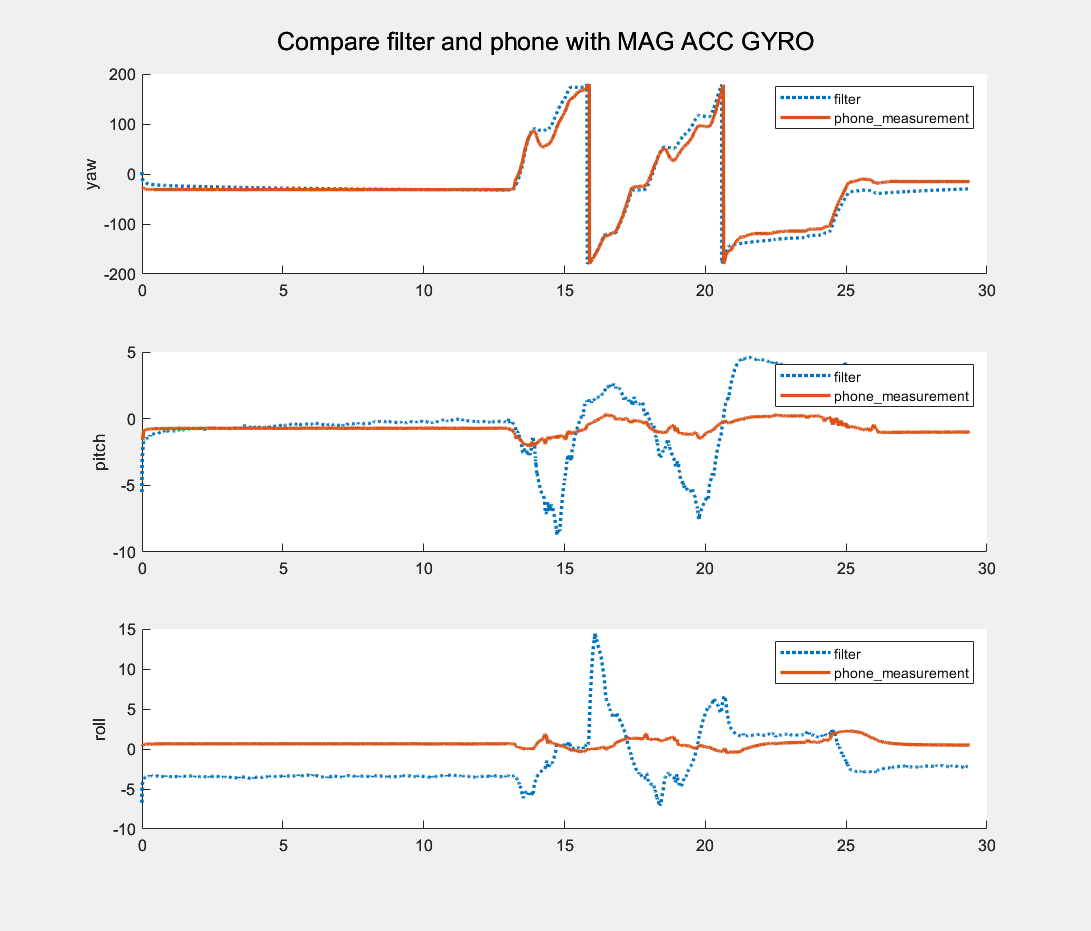
\includegraphics[width=0.7\textwidth]{images/allsensor3.png}
 \caption{All sensors: 3}
 \label{all3}
\end{figure}

From the three experiments, it can be observed that when all the sensors (mag, acc, gyro) are enabled, our designed filter performs relatively well in tracking rotations around the x-axis and y-axis. However, when facing rotations around the z-axis, except for the yaw angle, the tracking performance for the other two angles is very poor.

\subsection{Acc and Gyro}

\begin{figure}[H]
 \centering
 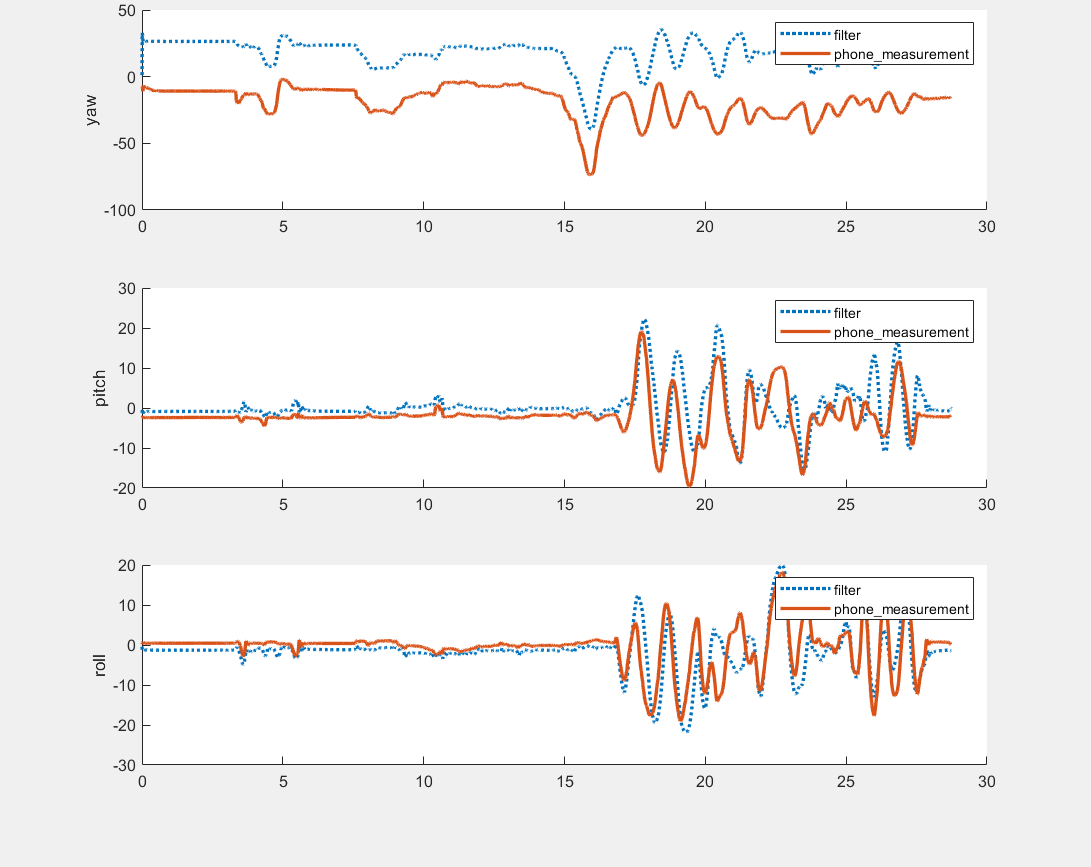
\includegraphics[width=0.7\textwidth]{images/accgyro.png}
 \caption{Acc and Gyro : complex}
 \label{accgyrocomplex}
\end{figure}

From figure \ref{accgyrocomplex}, it seems that without the magnetometer, the estimate result works really bad in yaw.

So test the special rotate for yaw:

\begin{figure}[H]
 \centering
 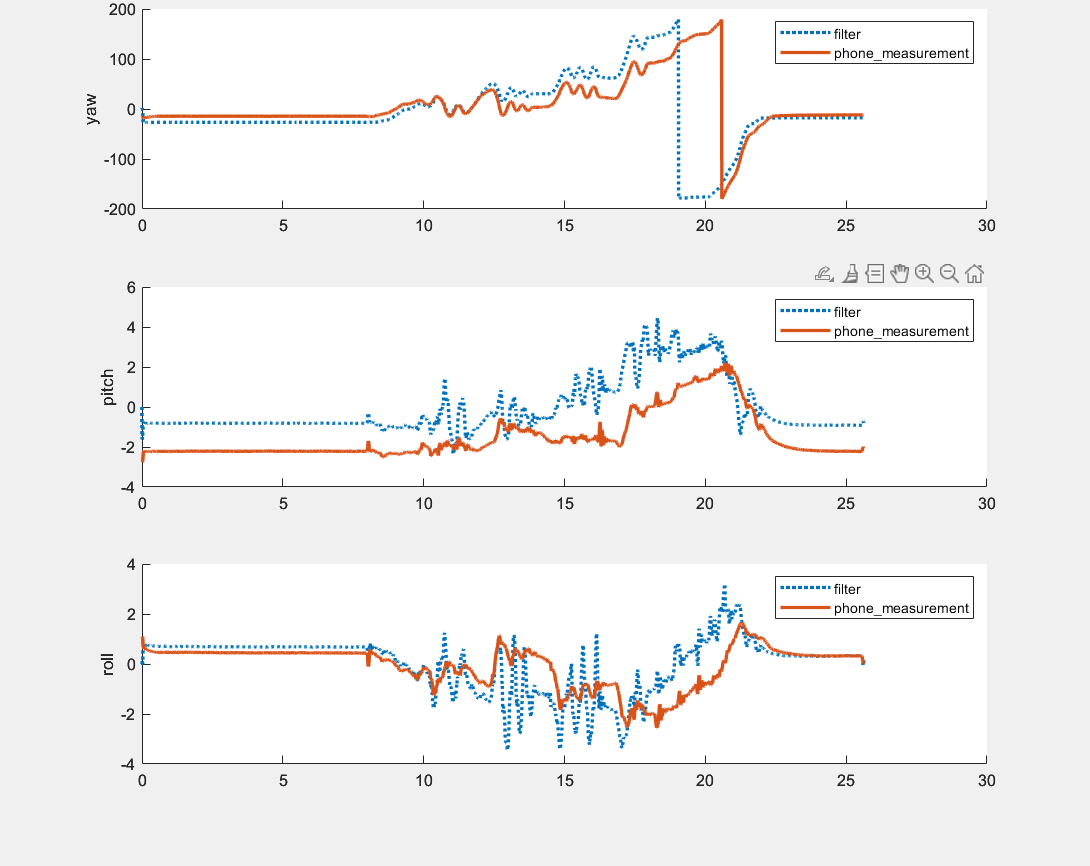
\includegraphics[width=0.7\textwidth]{images/accgyro2.png}
 \caption{Acc and Gyro : 3}
\end{figure}

It is difficult to evaluate whether the performance in the current situation is better than having the magnetometer present, since it seems catch more information than previous.

\begin{figure}[H]
 \centering
 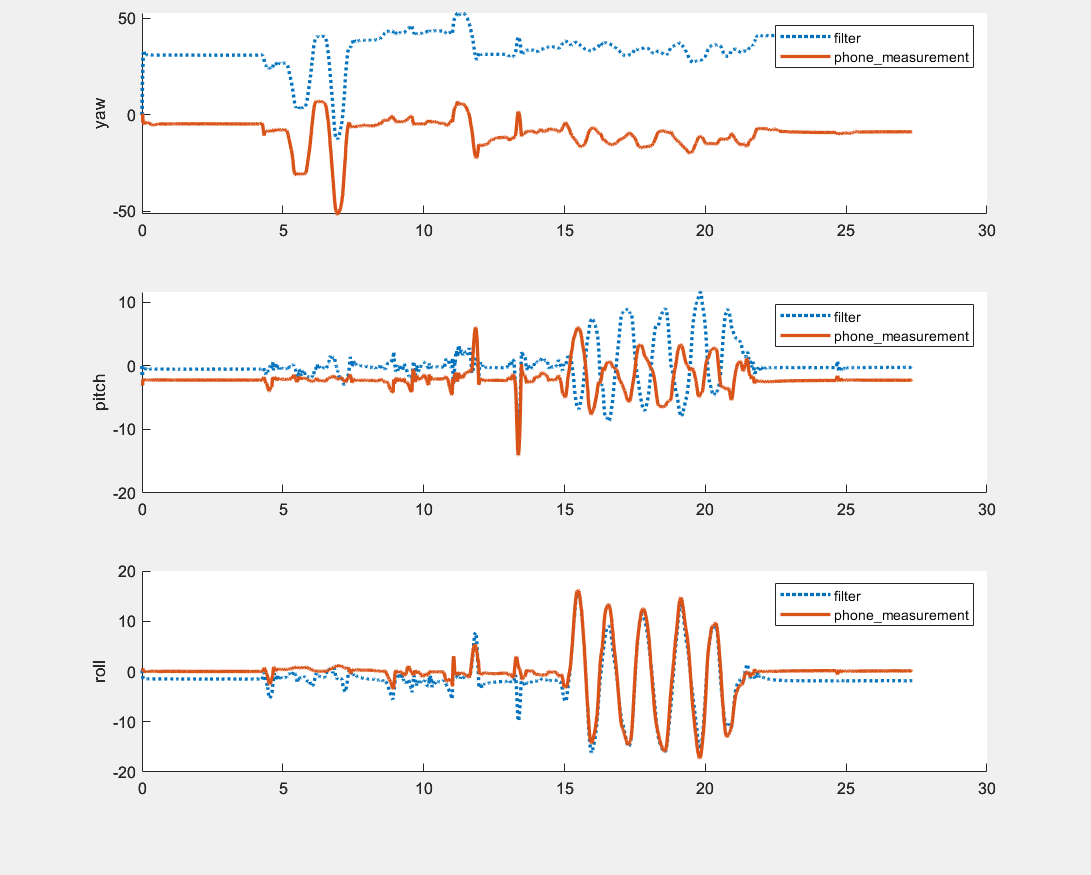
\includegraphics[width=0.7\textwidth]{images/accgyro1.png}
 \caption{Acc and Gyro : 1}
 \label{ag1}
\end{figure}


\begin{figure}[H]
 \centering
 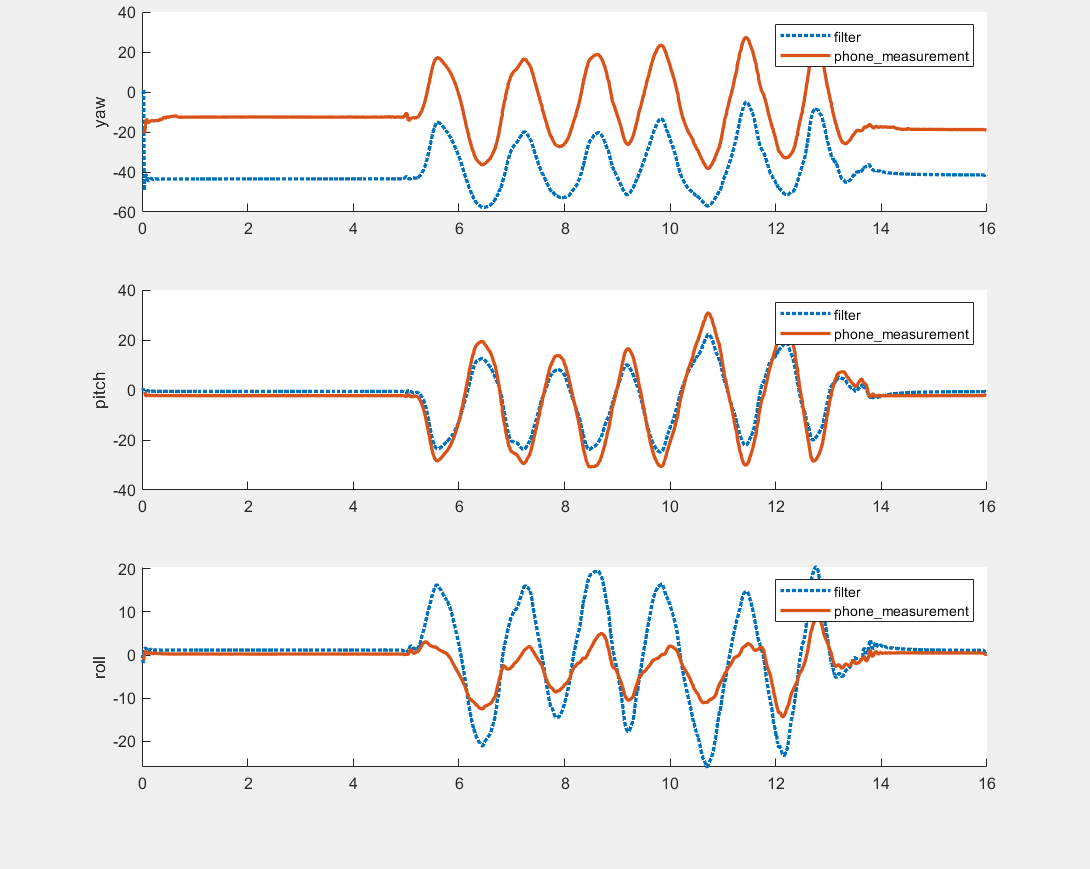
\includegraphics[width=0.7\textwidth]{images/ag2.png}
 \caption{Acc and Gyro : 2}
 \label{ag2}
\end{figure}

From figure \ref{ag1} and figure \ref{ag2}, it can be observed that without the magnetometer, the phone has lost its ability to correct its offset in yaw. Additionally, the tracking speed has decreased, and it can only achieve good tracking performance on axes with significant and active changes.

\subsection{Acc and Mag}

\begin{figure}[H]
 \centering
 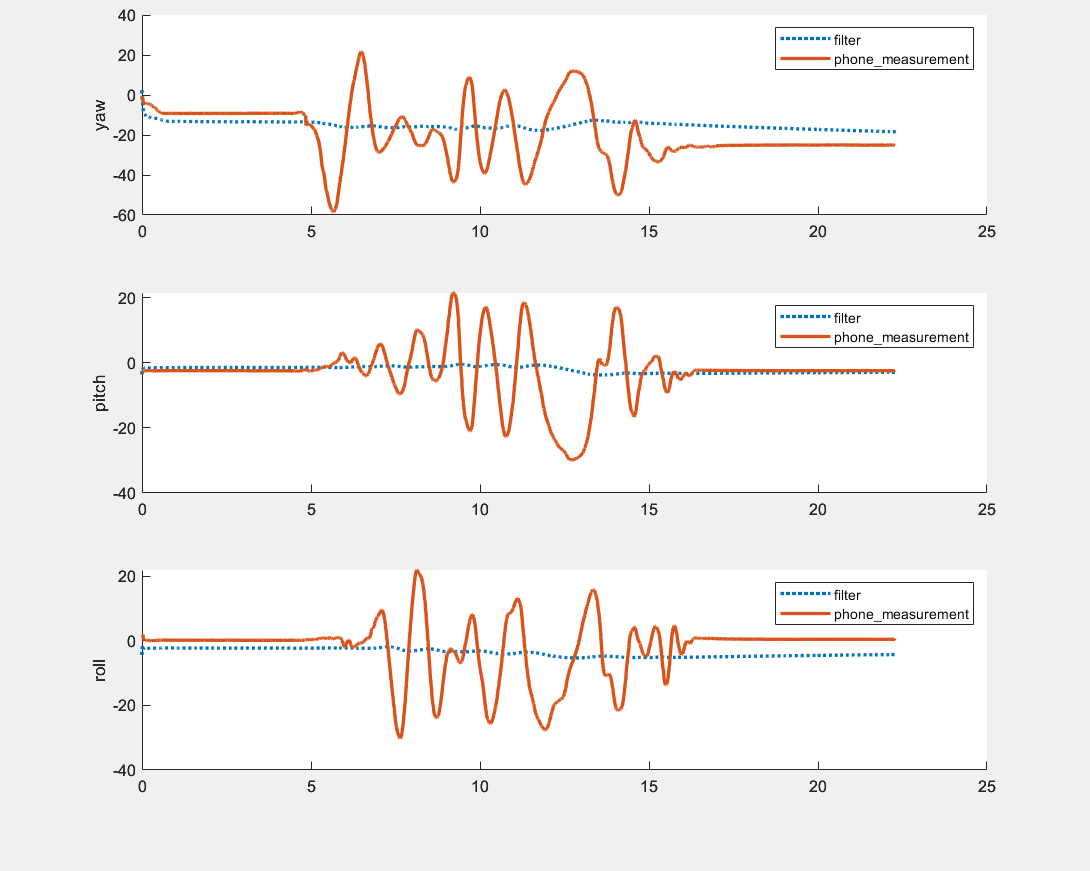
\includegraphics[width=0.7\textwidth]{images/accmag.png}
 \caption{Acc and Mag: complex}
\end{figure}

It can be observed that without the gyroscope, the filter is unable to function properly.

This is because without the gyroscope, the filter cannot accurately sense the device's rotation, leading to the inability to estimate the attitude. While the magnetometer and accelerometer can provide some information about the device's orientation, their measurement range is limited and susceptible to external interference. Without the angular velocity measurements provided by the gyroscope, the filter cannot effectively fuse and estimate the orientation using these sensor data.

Therefore, without the gyroscope, the filter lacks angular velocity information and is unable to perform accurate attitude estimation, resulting in its inability to function properly and being paralyzed.

\subsection{Gyro and Mag}

\begin{figure}[H]
 \centering
 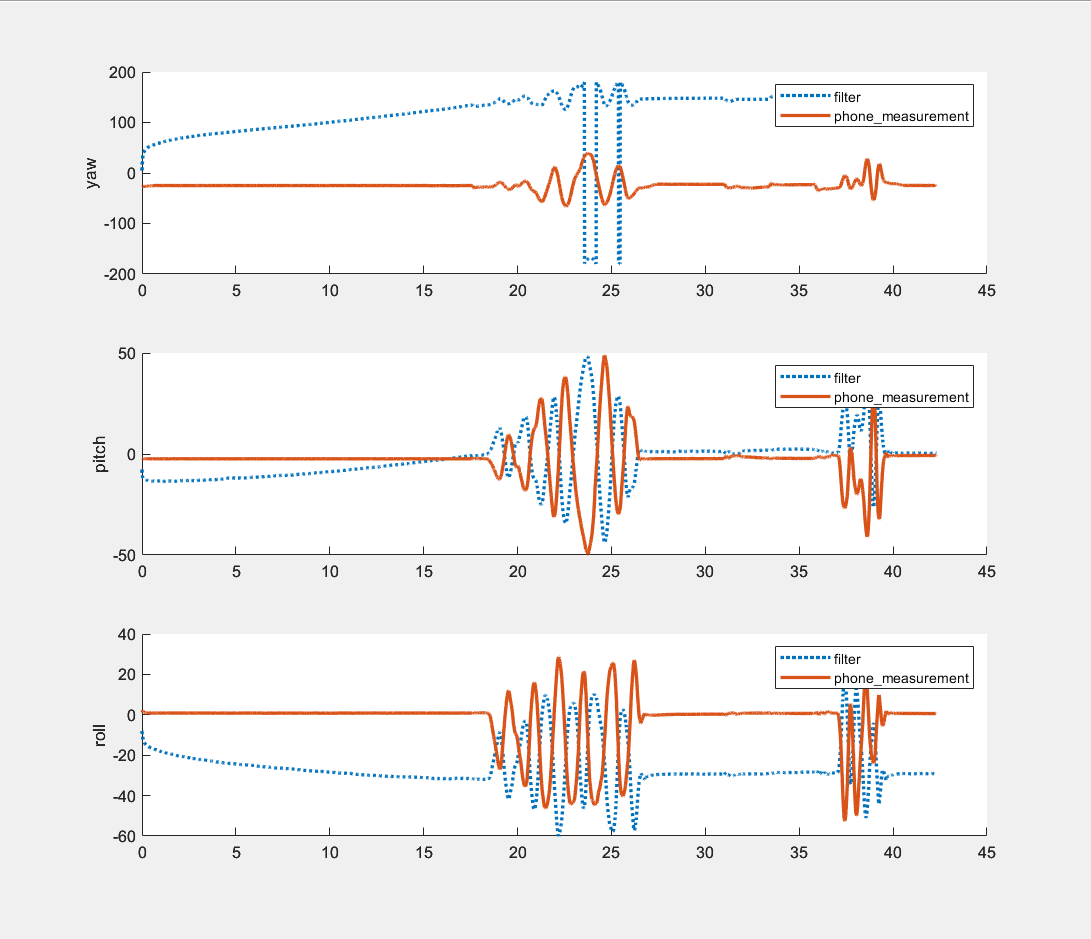
\includegraphics[width=0.7\textwidth]{images/Gyroandmag.png}
 \caption{Gyro and Mag: complex}
 \label{gmcomplex}
\end{figure}

\begin{figure}[H]
 \centering
 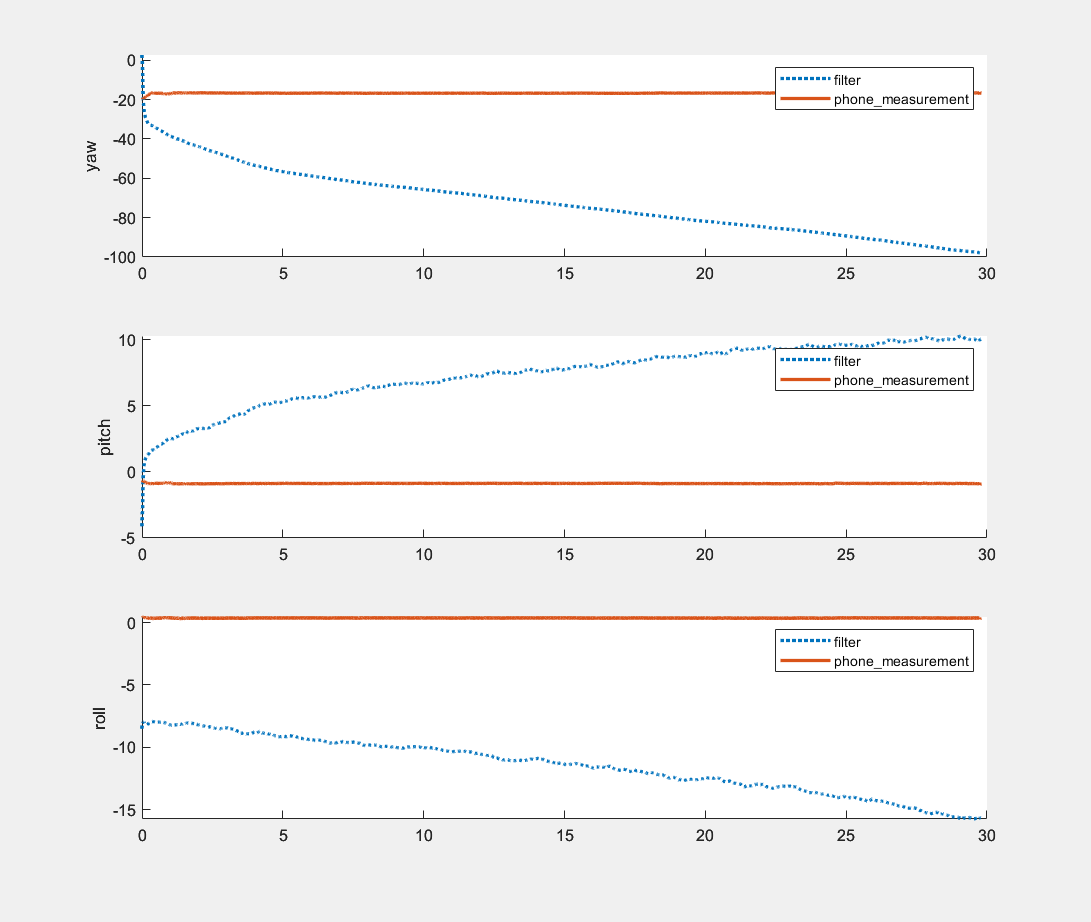
\includegraphics[width=0.7\textwidth]{images/gyromagflat.png}
 \caption{Gyro and Mag: flat}
 \label{flat}
\end{figure}

It has been observed that without the accelerometer, the device's attitude experiences continuous drift. This drift is primarily caused by the continuous updates from the magnetometer. Although the gyroscope can accurately perceive angular velocity, its measurements do not have practical significance due to the incorrect orientation of the coordinate axes. As a result, the gyroscope measurements are unable to salvage the performance of the filter.